\chapter{Implementierung}
\label{ch:implementierung}

\section{Server}
\label{impl:server}
Der Server hat die Aufgabe, die gesamte Kommunikation zwischen Controllern und Robotern zentral zu verwalten und zu koordinieren. Außerdem müssen die Eingabe und Ausgabe der Peripheriegeräte verwaltet, bzw. gesteuert werden. Diese Peripheriegeräte sind die Ladestation, die gefunden werden muss, die Torerkennung, die verarbeitet werden muss und die Infrarot-LED, mithilfe der die Ladestation gefunden werden kann. Auch die Bilddaten, die vom Roboter versendet werden, müssen hier zwischengespeichert werden und anschließend an die Controller weiter gegeben werden.

Als Hostgerät für den Server wurde ein RaspberryPi ausgewählt. Dieser bietet volle Unterstützung für Java-Programme und bietet mit seinen GPIO-Pins eine optimale Basis für die Ansteuerung und Überwachung der Peripheriegeräte. 
Als Programmiersprache wurde Java gewählt.


\subsection{Verbindung}
Die Verbindungslogik besteht im Wesentlichen aus fünf Klassen, die in Abbildung \ref{fig:verbindung} dargestellt sind. Verwaltet werden die Verbindungen in der Klasse ConnectionManager, der die Verbindungen für die Spiellogik bereit stellt, sobald ein Controller-Roboter paar verbunden wurde. Für die Verbindungen der Controller gibt es WebsocketSocket. Ein Objekt dieser Klasse dient als Schnittstelle der Kommunikation zwischen einem Controller und dem Server. Für die Verbindungen der Roboter gibt es UDPConnectionHandler. Auch ein Objekt davon steht für genau eine Verbindung mit einem Roboter. Um eine Verbindung mit einem Roboter herzustellen, wird in der Klasse UDPSocketProvider auf Port 44044 auf eingehende Pakete gewartet und anschließend ein Socket zu diesem Endpunkt bereit gestellt. Auch die Authentifizierung wird in dieser Klasse abgehandelt. Zusätzlich gibt es für den UDPConnectionHandler eine Hilfsklasse, die ConnectionControl. In dieser wird festgelegt, wie lange die Verbindung als offen gekennzeichnet werden soll, obwohl kein Paket ankommt. Auf der Controllerseite wird eine solche Implementierung nicht benötigt, da der WebSocket auf HTTP und damit auf TCP basiert. Ein Verbindungsabbruch ist dort auch ohne Timeout erkennbar.


\begin{figure}[h]
	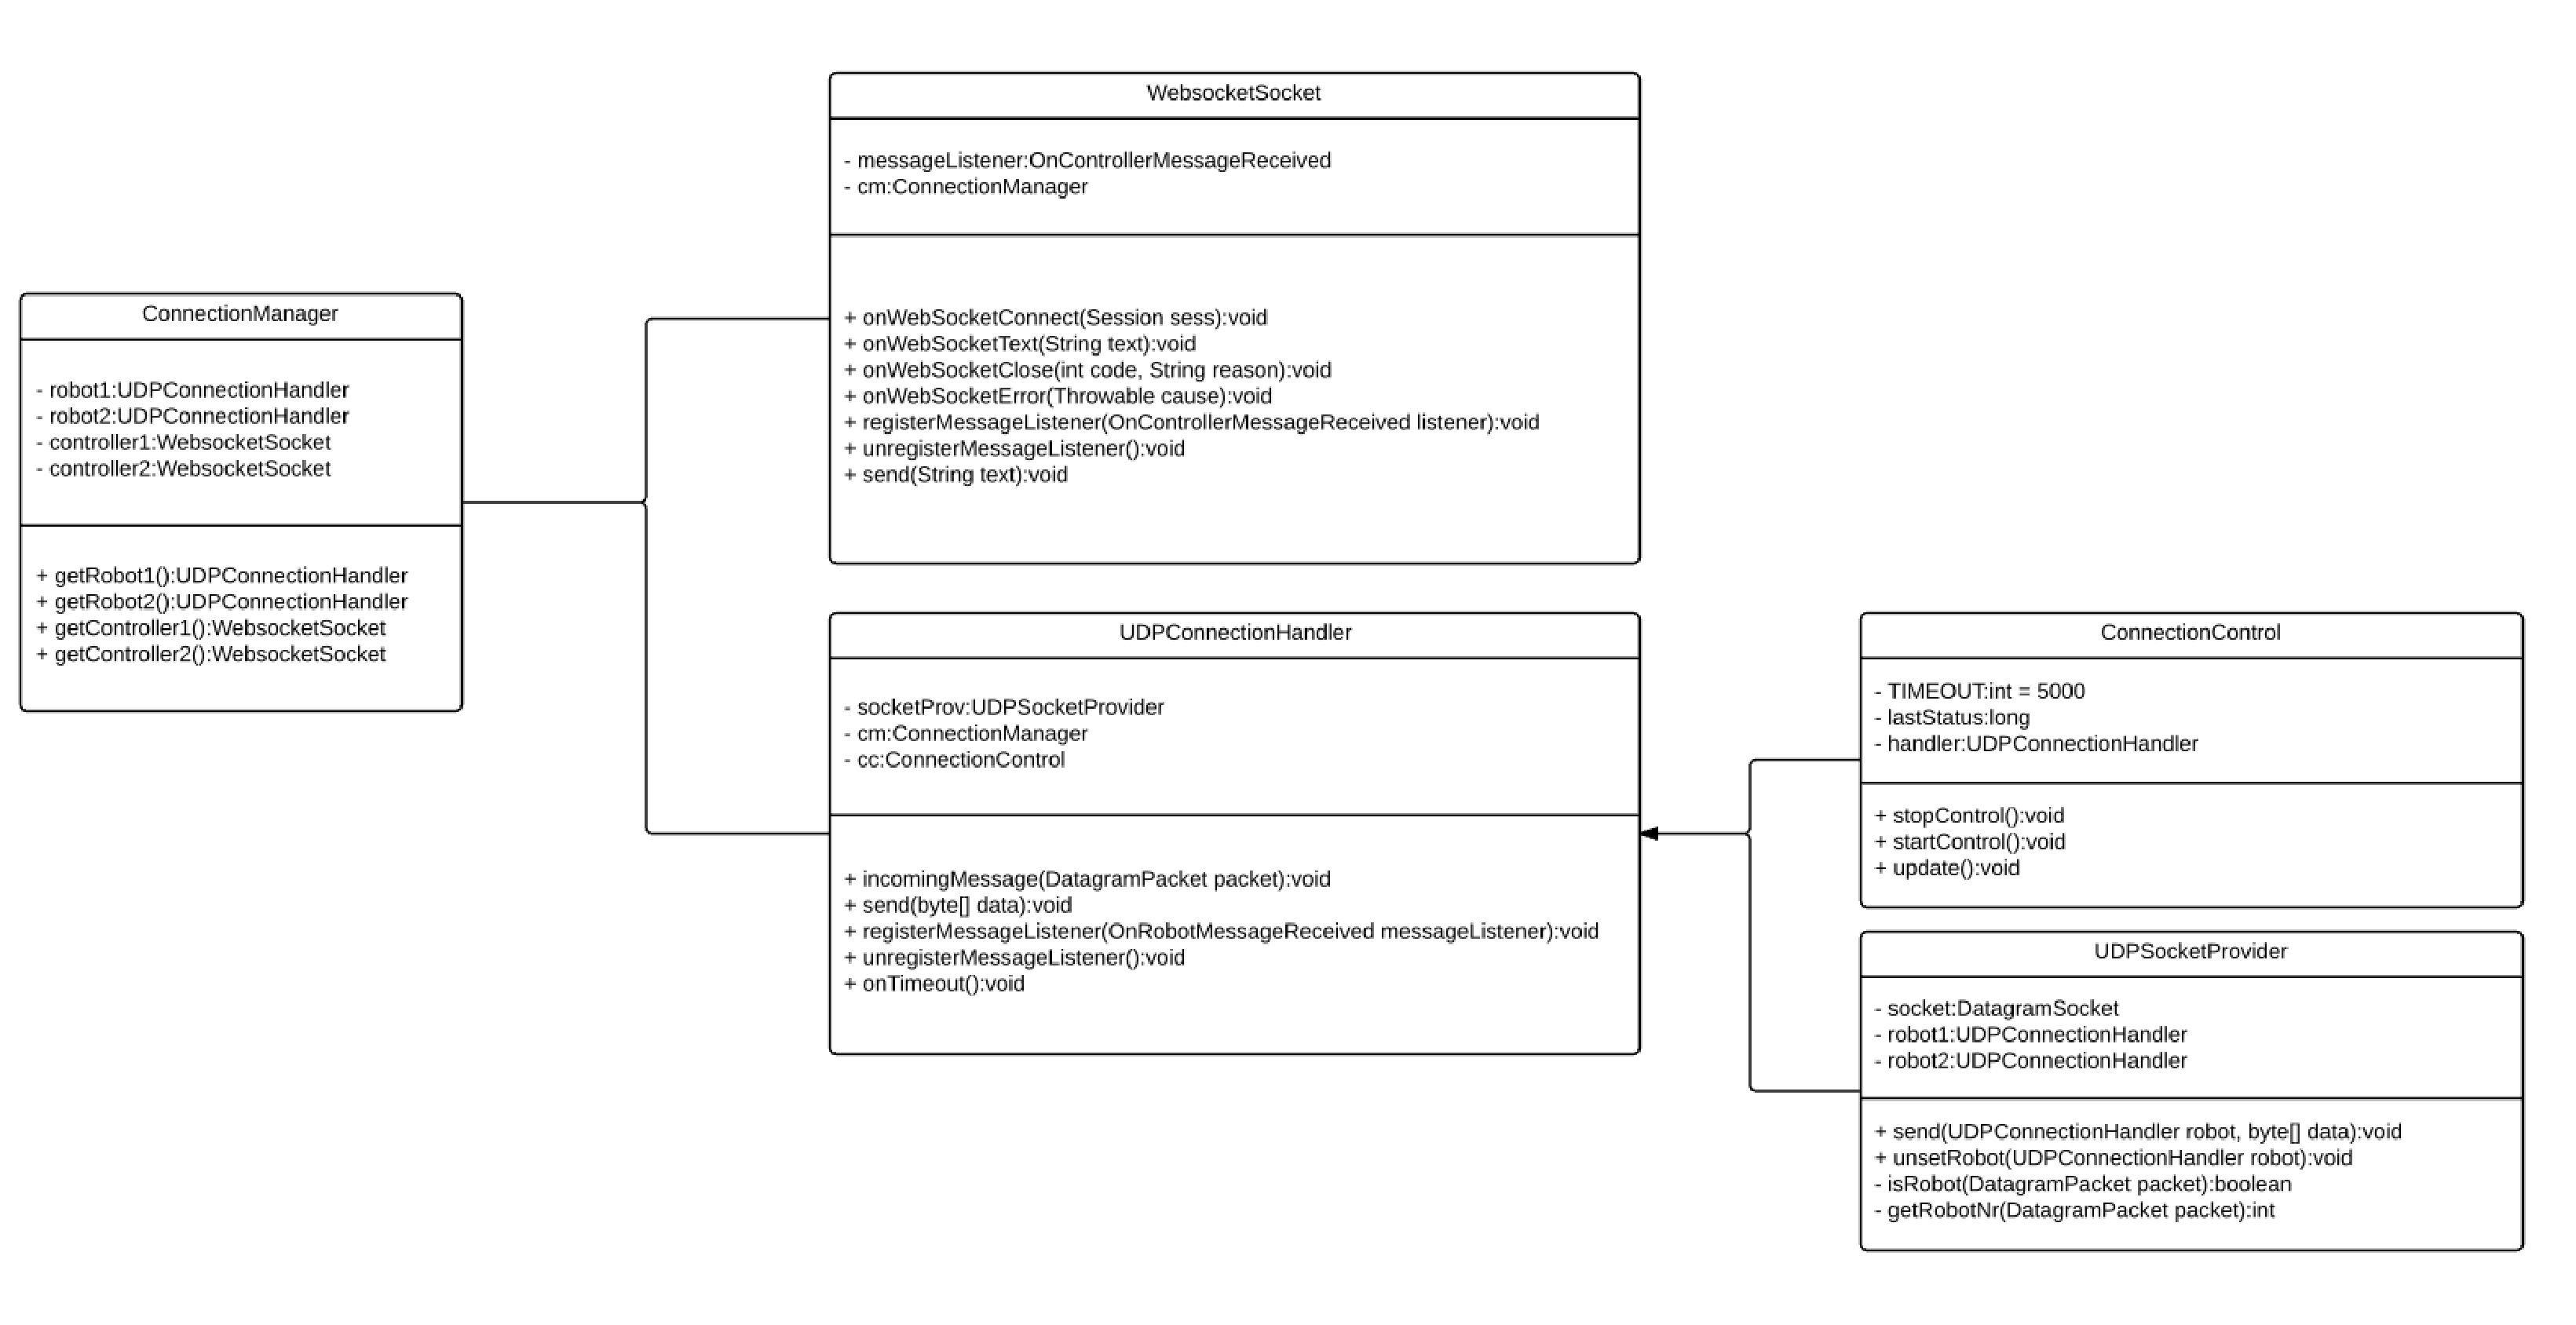
\includegraphics[width=\textwidth]{images/uml_verbindung.pdf}
	\caption{Klassendiagramm der Verbindungslogik}
	\label{fig:uml_verbindung}
\end{figure}



\subsection{Bildübertragung}
Wie in der Schnittstellenbeschreibung in Abschnitt \ref{sec:schnittstelle} beschrieben, werden die Bilddaten vom Roboter an die Statusnachrichten angehängt. Hierbei kennzeichnen die Bytes FF D8 den Beginn eines neuen Frames. Diese Kombination tritt in JPEG-kodierten Bildern immer nur am Anfang des Bildes auf, wodurch es möglich ist, Bilddaten über mehrere Pakete zu verteilen. Diese Daten werden dann in der Player-Klasse gepuffert, bis das Bild vollständig ist. Anschließend wird es noch base64 kodiert und sofort an die Controller weiter gesendet. Die base64 Kodierung wurde im Gegensatz zur einfachen Byte-Orientierten übertragen bevorzugt, damit an mit den Controllern in einer höheren Datenabstraktionsebene kommuniziert werden kann. Das vereinfacht den Code vor allem in der Webanwendung, da diese in Javascript implementiert ist. Ein großer Nachteil dieser Kodierung ist der größere Speicherbedarf, der die Übertragung aufgrund höheren Traffics langsamer macht und dadurch zu Verzögerungen führt, die letztendlich im Verlust der Steuerbarkeit resultieren können. Nach ersten Tests ist die Bildrate vom Roboter jedoch so gering, dass diese wenigen Frames rechtzeitig übertragen werden können. Zusätzlich sind die Frames in einer Größenordnung, in der 33 \% Mehrbedarf noch zu keiner Netzwerküberlastung führen.



\subsection{Torfindung}
Über die Statusmeldungen des Roboters erfährt der Server wie hoch der Akkustand des Roboters ist. Sobald der Roboter ein Minimum des Akkustands unterschreitet, greift die Torfindung ein. Diese wird in der Klasse EnergyManager implementiert (siehe Abb. \ref{fig:uml_energymanager}). Dabei wird die Torfindung sofort aktiviert, wenn sich ein Roboter mit dem Server verbindet und nicht erst wenn noch ein Controller hinzu kommt. Über das "seeGoal" Flag (vgl. Schnittstellenbeschreibung \ref{sec:schnittstelle}) kann erkannt werden, ob das zum Roboter gehörende Tor in Sicht ist. 
%TODO hier weiter machen mit den LEDs, bzw. verweisen auf die infrarot led ladestation section. 

\begin{figure}[h]
	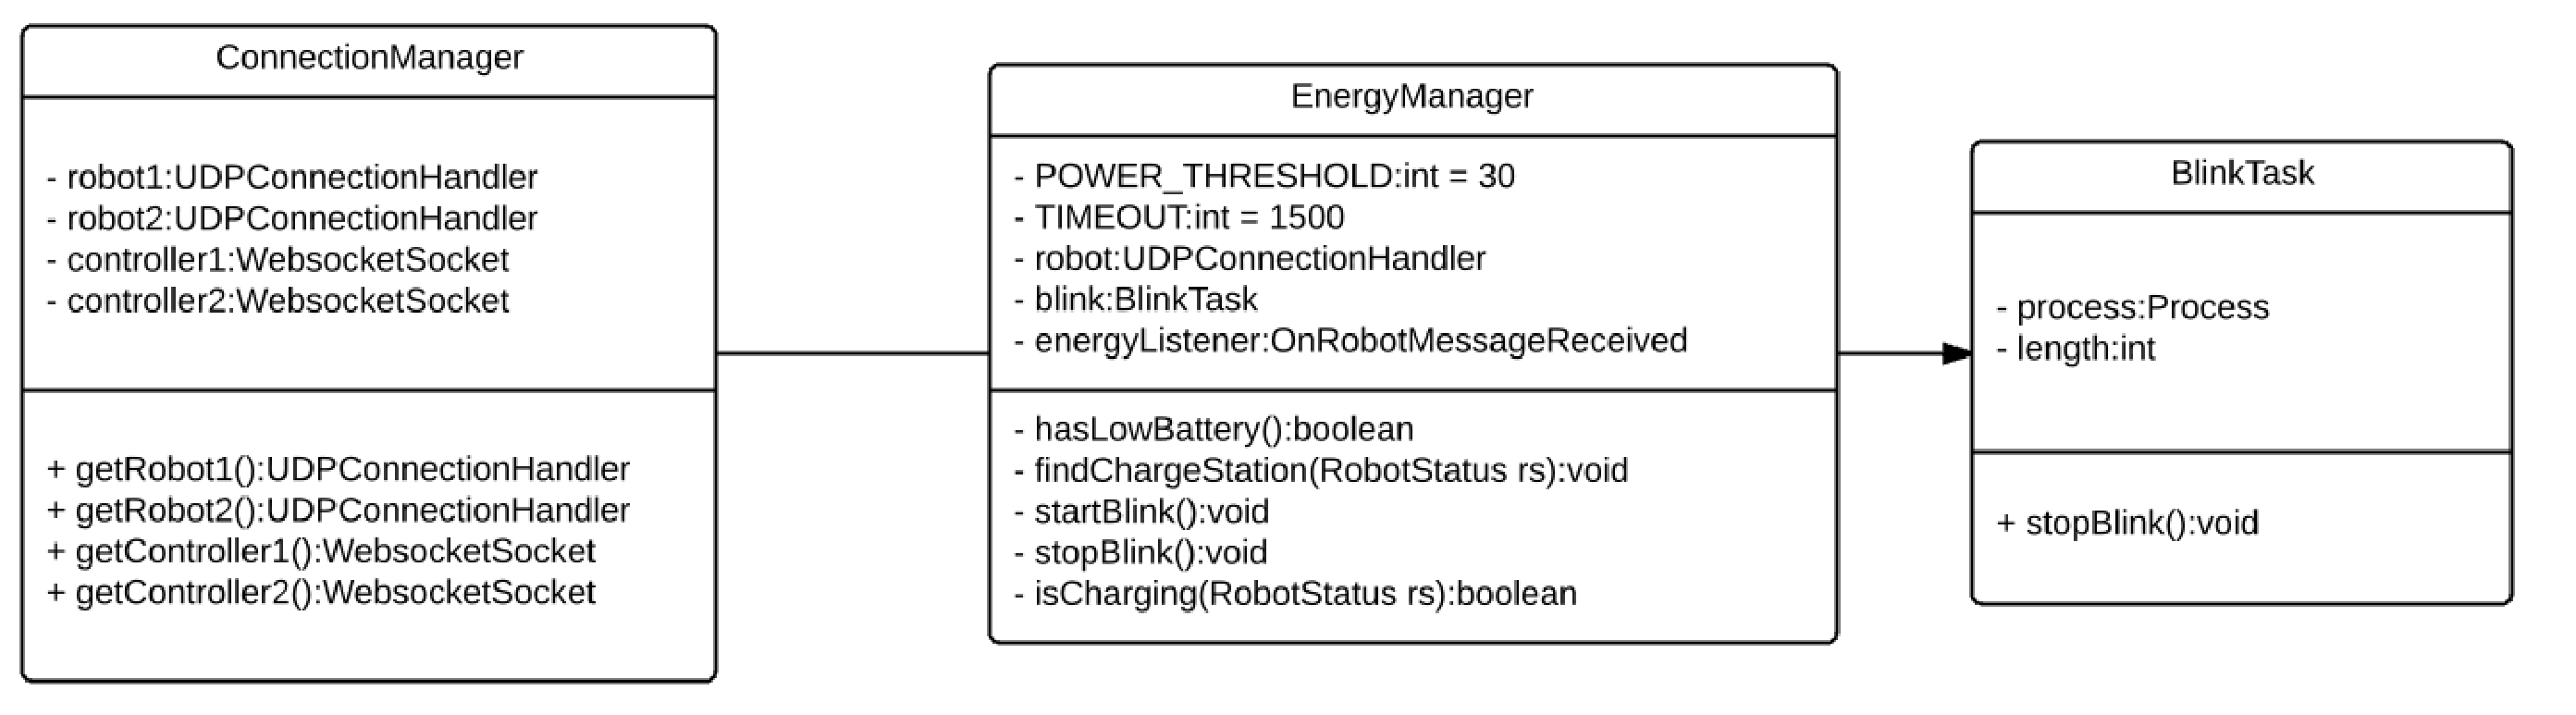
\includegraphics[width=\textwidth]{images/uml_energymanager.pdf}
	\caption{Klassendiagramm der Torfindung}
	\label{fig:uml_energymanager}
\end{figure}

\section{Ladestation}
\subsection{Infrarot-LED}
\label{sec:infrarot_led}
\subsection{Torerkennung}

\section{Webanwendung}

\section{Android-Anwendung}
\subsection{RC-Remote Steuerung}
\subsection{Differential Steuerung}

